% Slides 2--4: motivation, scope, and research questions.

\begin{frame}{Hans made the risk visible}
  \begin{columns}[T,onlytextwidth]
    \begin{column}{0.44\textwidth}
      \begin{itemize}
        \item Extreme rainfall affected Southern and Eastern Norway in August 2023
        \item National precipitation was 45\% above the August normal
        \item More than 100 local precipitation records were set
        \item Warnings covered precipitation, flooding and landslides
      \end{itemize}
    \end{column}
    \begin{column}{0.53\textwidth}
      % Replace with an English-labelled or licensed version when available.
      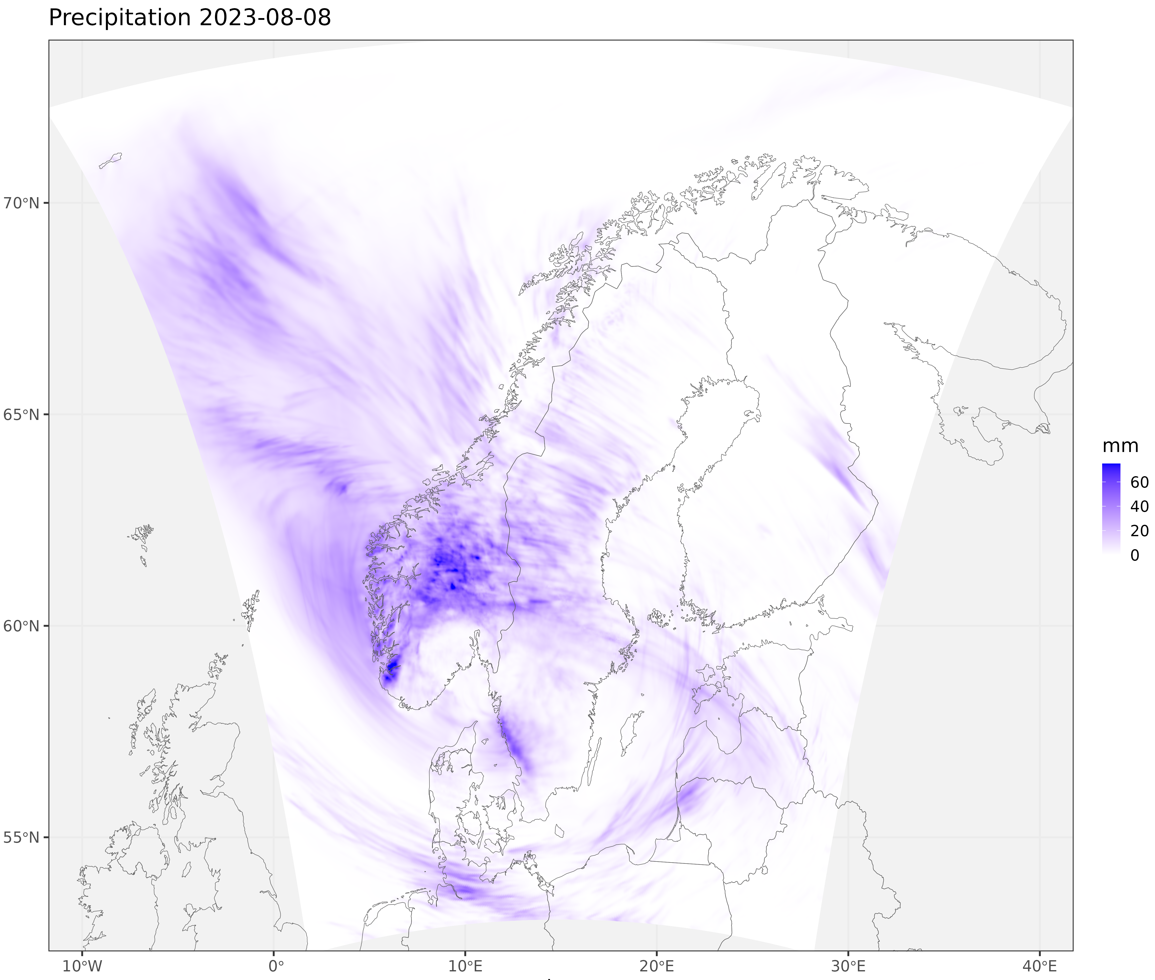
\includegraphics[width=\linewidth,height=0.61\textheight,keepaspectratio]{images/storm-hans.png}
    \end{column}
  \end{columns}
  \sourceNote{Norwegian Meteorological Institute (2023)}
\end{frame}

\begin{frame}{The hazard we model is not river flooding}
  \begin{columns}[T,onlytextwidth]
    \begin{column}{0.53\textwidth}
      \textbf{Included: pluvial water damage}
      \begin{itemize}
        \item Rain or snowmelt entering from outside
        \item Sewer backflow from overloaded drainage
        \item Water entering through the building envelope
      \end{itemize}

      \textbf{Excluded}
      \begin{itemize}
        \item Rivers or lakes overtopping their banks
        \item Claims classified as natural-hazard flooding
      \end{itemize}
    \end{column}
    \begin{column}{0.42\textwidth}
      \textbf{Different mechanisms}
      \begin{itemize}
        \item Pluvial risk depends on local rainfall, drainage and the building envelope
        \item River-flood risk depends on upstream flow, channel capacity and floodplain exposure
      \end{itemize}
    \end{column}
  \end{columns}
  \sourceNote{Gjensidige claims data; Finans Norge (2025)}
\end{frame}

\begin{frame}{Two motivations, one modelling framework}
  \begin{columns}[T,onlytextwidth]
    \begin{column}{0.57\textwidth}
      \begin{enumerate}
        \item \textbf{Climate adaptation}
          \begin{itemize}
            \item Quantify changes in expected damage costs
            \item Compare mid- and late-century horizons
          \end{itemize}
        \item \textbf{Insurance insight}
          \begin{itemize}
            \item Identify drivers of claim frequency and severity
            \item Improve the representation of short-duration rainfall
          \end{itemize}
      \end{enumerate}
    \end{column}
    \begin{column}{0.38\textwidth}
      \textbf{Common framework}
      \begin{itemize}
        \item Building-level risk model
        \item Relative cost changes
        \item Building and precipitation effects
      \end{itemize}
    \end{column}
  \end{columns}
  \sourceNote{Norwegian Expert Committee on Climate Adaptation; Gjensidige}
\end{frame}
